\chapter{Technology and Software}
In this chapter we discuss the technology that will be used to implement our solution. Android, Playstation Move and Wii Remote are described in detail. We also look at existing applications with similar functionality to our own system. 

\section{Android OS}
Android is a Linux based operating system primarily designed for touchscreen devices such as smartphones and tablets. It is developed by Google and is supported by The Open Handset Alliance (OHA). The source code was released as open source under the Apache License, and The Android Open Source Project is tasked with maintaining and further developing the operating system. The OHA is a consortium focused on developing open standards for mobile devices, and members of the consortium are not allowed to produce phones that are not compatible with the Android OS. Applications for the Android OS are primarily written in a customized version of Java using the Software Development Kit, but it is possible to partly write applications in C and C++ using the Native Development Kit. 

Given that the Android OS code is open source and highly modifiable both the community and smartphone distributors have taken advantage of this. Smartphone producers such as HTC and Samsung have made their own versions of the Android OS. These versions come preinstalled on the devices and are referred to as stock firmware. The modifications are primarily focused on making the user interface more powerful and user friendly in order to enhance the user experience \cite{htcSense}. The Android community has also developed their own versions of the Android OS. This firmware might be specialized to be lightweight, or allow a high degree of customization to better suit advanced users. The best known and most complete community firmware is the CyanogenMod \cite{cyanogenMod}. In order to install and use custom firmware a user needs to ``root’’ the phone. Rooting the phone gives the user access to the entire system, allowing the old firmware to be removed and the new community firmware to be installed.

The software center for Android is known as ``Google Play’’ and allows developers to easily distributed their applications. Users can then choose and download thousands of applications, some are free, while others have to be paid for. The idea is that as long as a device runs the Android OS it can run any of the applications on Google Play. The first Android device was sold in October 2008. By the end of 2010 the Android OS had become the leading smartphone platform \cite{androidLeadingPlatform}, and at the second quarter of 2012 it had a worldwide smartphone market share of 68\% \cite{androidMarketShare}. During the third quarter of 2012, 500 million devices had been activated and there are approximately 1.3 million activations per day \cite{androidDevices}. As of writing, the newest Android version is 4.1, codename Jelly Bean. Figure~\ref{fig:verDist} shows how the different versions are distributed on existing Android smartphones. As the figure shows, most devices have not been updated to the latest version, either because of hardware limitations or because the stock firmware has not been updated by the vendor. With each new version of Android the developer API is improved and functionality is added. Applications using a lower API level developed for earlier Android versions can run on higher API levels, but not the other way around. Using a lower level API allows an application to support more devices, but sacrifices added features and optimization located in a higher level API.

\begin{figure}[h!]
  \centering
    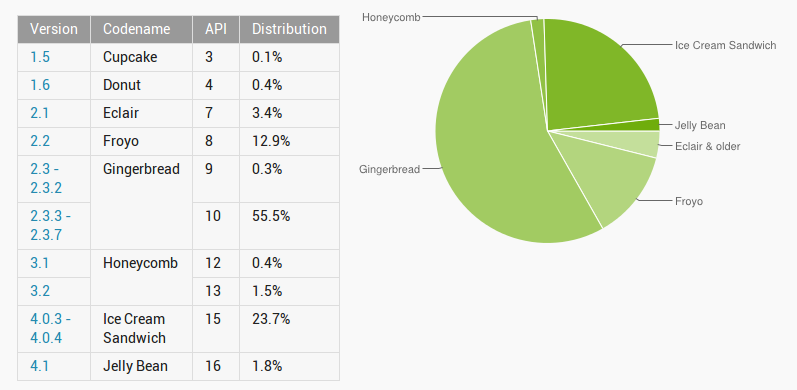
\includegraphics[width=1.0\textwidth]{androidVersionDistribution.png}
    \caption{\footnotesize Version distribution as of October, 2012. The data is based on Android devices that accessed Google Play during a 14 day period \cite{androidVersions}}
  \label{fig:verDist}
\end{figure}

\subsection{Architecture}
Older Android versions are based on Linux kernel 2.6 while Android version 4.0 and higher use Linux kernel 3.0. Google has made alterations to the standard Linux kernel by not including all the standard libraries (see figure~\ref{fig:androidArchitecture}), this makes porting existing Linux desktop applications difficult. The kernel interacts with the hardware and contains all the necessary drivers in order to do so. As the operating system was designed to run on a variety of hardware, the kernel functions as an abstraction layer between the hardware and software in addition to handling the standard kernel tasks such as resource management, networking and security.

\begin{figure}[!h]
  \centering
    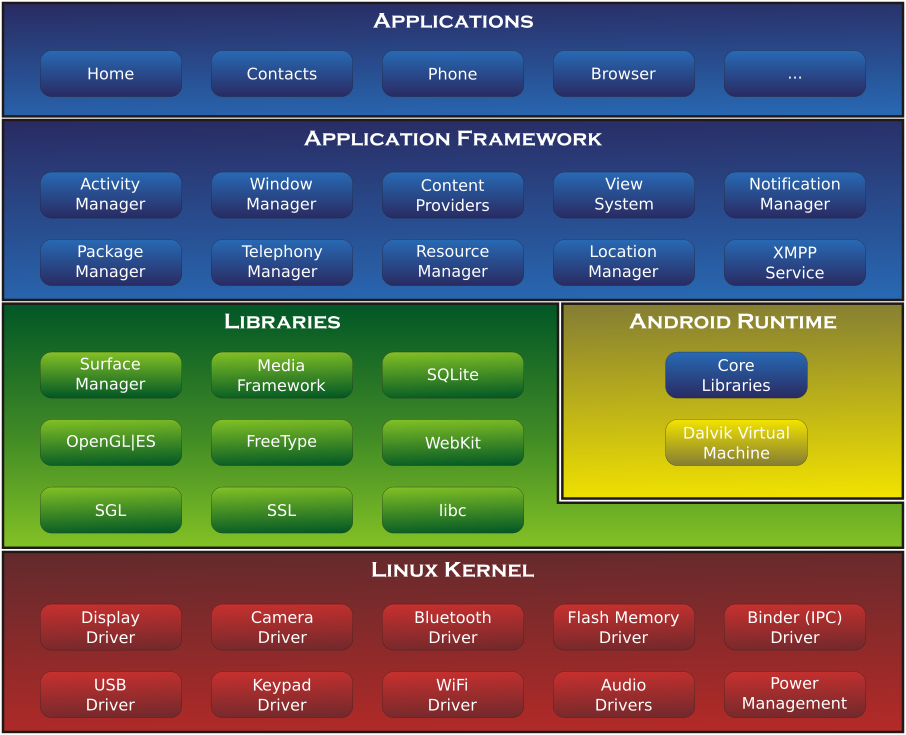
\includegraphics[width=1\textwidth]{androidArchitecture.png}
    \caption{\footnotesize A visual representation of the Android architecture}
 \label{fig:androidArchitecture}
\end{figure}

The library layer contains the native android libraries that enable android devices to handle different types of data. The libraries are written in C++ or C and are hardware specific. These libraries can be accessed through the use of the Android NDK and is recommended for functionality not attainable through the standard SDK. There are dozen of native libraries but some of them include: Webkit is the browser engine used to display HTML content, SQLite is used for data storage locally on the device, OpenGL to render 2D and 3D graphics, in addition to several media codecs. Google has developed their own Java Virtual Machine called the Dalvik Virtual Machine. It runs Android applications and is optimized for low memory and low processing power environments. It provides most of the same features as the JVM such as isolation, multi-threading and memory management. The DVK in addition to core java libraries are called the Android Runtime.

The Application Framework level is what applications on the Android device interact with. Developers use the programs located in this framework as tools to build their own applications. These programs provide access to and manage basic phone functions, such as GPS tracking (Location Manager), sharing data between applications(Content Providers) voice calls (Telephone Manager), applications lifecycles (Activity Manager) and so on. Any application installed by the user is located in the top application layer. These are applications created by developers and can range from SMS clients, to 3D games.

\section{Existing Applications}
The Google Play Store contains a handful of applications that enable an Android device to be connected to a Wii Remote through Bluetooth. The majority of these applications only provide basic features such as key presses, led lights, and rumbling \cite{wiimoteController, simpleWiiController}. There was one application that stood out and utilized the motion detection features of the Wii Remote and gave the sense of a complete application. Wii Motion Monitor \cite{wiiMotionMonitor} turns the Wii MotionPlus into a motion sensor, and is able to represent the orientation of the Wii Remote correctly. Yaw was off by about 45 degrees, but pitch and roll worked perfectly. This proves that the Wii Remote can be used for motion detection and an Android device can act as a hub.

There was only one application \cite{sixaxisController} that enabled a user to connect a SixAxis Playstation 3 controller to an Android device. The application requires root access, and additional work had to be done before the controller was ready to be paired. A compatibility checker is available to see if an Android device is compatible with the software.

\section{Playstation Move}
This section looks closer at the Playstation Move controller. First we will look at the hardware and relevant sensors that we can utilize. Second we will look at relevant libraries that can be used to establish a connection to the controller.

\subsection{Motion Controller Hardware}
The PS Move motion controller contains advanced motion sensing, making it an ideal peripheral for a biofeedback system. It features three different types of sensors: accelerometer, gyroscope and magnetometer. Accelerometer and gyroscope is used for motion tracking, and the magnetometer provides the horizontal orientation based on the earth’s magnetic field. The built in vibration and orb light can be used to provide feedback to the user \cite{psMoveTech}. Unlike the Wii Remote it uses built-in batteries that can be charged using a USB-mini cord. 

\subsection{PS Move API}
The PS Move API \cite{PSMoveAPI} is written in C, but contains bindings for various languages, including Java and C\#. Both of these languages are used in smartphone application development. The API explicitly mentions that it runs on Android devices.This is only partially true: It will not run out of the box on an Android device, restructuring and heavy modification of the Android device is required. The Android OS runs on top of a modified Linux kernel, this kernel does not contain the necessary libraries and drivers in order for the API and Motion controller connectivity to function properly. The next step would be to compile the C API into a shared library using the Android NDK, and use the shared library Java bindings in the Android Java code. The lead developer has implemented a working application on a smartphone with a custom kernel, but states that due to the Android kernel he is having a hard time making it work ``out of the box’’ and is only a proof of concept. The API is still in development as of writing.

Because of the technical challenges and the lack of documentation on the reverse engineering of the Playstation Move, it was decided that the Wii Remote was a better choice for the controller. If the API was more mature, and the Android kernel had more drivers it would have been viable. An alternative approach would be to use a smartphone running Ubuntu, which is currently under development \cite{ubuntuAndroid}.

\section{Wii Remote with MotionPlus}
In this section we present the Wii Remote and MotionPlus hardware, and describe some of the third-party libraries that exist for connecting to the device.

\subsection{Wii Remote and Motion Plus Hardware}
The original Wii Remote features motion tracking for vertical movement, left-right horizontal movement, and horizontal rotation through the use of an ADXL330 accelerometer.\cite{wiiAccelerometer}. In June 2009 Nintendo released the Wii MotionPlus expansion device which contains a dual-axis tuning fork and a single-axis gyroscope\cite{wiiMotionPlus}. The expansion device improves the motion tracking of the Wii Remote greatly, but makes it larger. Nintendo has now started selling the Wii Remote Plus. It is the same size as the Wii Remote, but has the Wii MotionPlus already built in. Both of the controller types have the ability to provide vibration and basic audio feedback. The Wii Remote is powered by a pair of AA batteries.

\subsection{Wii Remote API}
At the time of writing no open source Wii Remote library has been published for the Android OS. Though some Wii Remote libraries exist, none of them are intended to be used on Android devices. The next subsections will cover the libraries that are implemented in Java.

\subsubsection{WiiRemoteJ}
WiiRemoteJ is one of the most complete libraries for the Wii remote. It is a pure Java library with support for a large amount of Wii extensions such as the Wii Guitar, and Wii Balance Board. It does however lack support for the MotionPlus extension. The library has not been update since July 2008. The author has taken down the homepage where the library was originally located, but it can be found on third party websites \cite{WiiRemoteJ}.

\subsubsection{WiiuseJ}
WiiUseJ is a lightweight Java API. It was built on top of the Wiiuse API and only supports the Wii Remote and the Nunchuck. Like the previous library it lacks support for the MotionPlus extension. The project has been discontinued since January 2009 \cite{Wiiusej}.

\subsubsection{Motej}
Motej is an open source (licensed under ASL 2.0) library for the Wii remote written in Java. Motej supports only the Wii Remote and IR Camera in its basic form. An extension library exists, adding support for the balance board, classic controller, and nunchuk. The project is currently at version 0.9, and was discontinued in 2009 \cite{Motej}.

\section{Bluetooth}
Bluetooth is a short-range communication technology that is simple and secure. The technology aims to provide a wireless alternative to cables when connecting two devices. Key features such as robustness, low cost, and low power consumption has made it one of the leading standards in its field and is supported by most modern operating systems through integrated hardware or portable Bluetooth adapters.

When a secure connection is established between two Bluetooth devices it is referred to as pairing. The devices can then securely communicate and transfer data with each other. Bluetooth is based on a master-slave architecture, allowing a single device to have up to 7 slaves, meaning that package exchanges are based on the masters clock. This is known as a piconet and a device can be a member of several piconets simultaneously. Bluetooth has three different classes of radios. The class specifies the range and power consumption of the radio. Most devices, including mobile phones and game controllers, use the Class 2 radio. Class 2 allows a range of at least 10 meters and consumes 2.5mW of power \cite{bluetooth}.

Bluetooth has a stack of different protocols. Android smartphones use the Radio Frequency Communications (RFCOMM) protocol. RFCOMM is based on the lower level Logical Link Control and Adaptation Protocol (L2CAP), and provides a reliable data stream with serial port emulation. Both Playstation Move and Wii Remote uses the L2CAP for communication. This low level protocol is not directly supported by the current version of Android, how we solved this issue is described further in the section~\ref{sec:motejOnAndroid}.